\documentclass[11pt]{article}
\usepackage[a4paper, total={7in, 8in}]{geometry}

\usepackage[backend=bibtex]{biblatex}
\addbibresource{bibliography}

\usepackage{multicol}

\usepackage{amsfonts}
\usepackage{amsmath}

\usepackage{xcolor}

\usepackage{graphicx}
\graphicspath{ {./images/} }

\usepackage{nameref}

\usepackage{lscape}

\usepackage{multicol}
\usepackage{multirow}

\usepackage{float}

\definecolor{mGreen}{rgb}{0,0.6,0}
\definecolor{mGray}{rgb}{0.5,0.5,0.5}
\definecolor{mPurple}{rgb}{0.58,0,0.82}
\definecolor{backgroundColour}{rgb}{0.95,0.95,0.92}
% ------------------------------------------------------------------------------
% minted
% ------------------------------------------------------------------------------
\usepackage{minted}

\newminted{python}{fontsize=\scriptsize, 
	linenos,
	numbersep=8pt,
	gobble=4,
	frame=lines,
	bgcolor=bg,
	framesep=3mm} 
% ------------------------------------------------------------------------------
% tikz
% ------------------------------------------------------------------------------
\usepackage{tikz}
\usetikzlibrary{calc, arrows.meta, positioning, automata, shapes}

\usepackage{listings}
\usepackage[most]{tcolorbox}
\usepackage{inconsolata}
\usepackage{float}

\usepackage[hidelinks]{hyperref}
\usepackage[justification=centering]{caption}

\newtcblisting[auto counter]{sexylisting}[2][]{sharp corners, 
	fonttitle=\bfseries, colframe=gray, listing only, 
	listing options={style = mystyle}, 
	title=\small Example \thetcbcounter: #2, #1,
}

\lstdefinestyle{mystyle}
{
	language = C++,
	basicstyle = \small,
	keywordstyle = {\bfseries},
	keywordstyle = [2]{\bfseries},
	keywordstyle = [3]{\scshape},
	otherkeywords = {endmethod, endclass},
	morekeywords = [2]{method, class, load, store, from, in},
	morekeywords = [3]{Profile, setFirstName, getFirstName, testSetFirstName, assertEq},
	emph = {var, p, profile, name, firstName, lastName},
	emphstyle=\itshape,
	literate = {=}{{$\gets$}}1,
	numbers = left,
	xleftmargin = 2.0ex
}

\title{\vspace{-3cm}Analysis of Focal Methods using Intermediary LLVM}
\author{Lars Van Roy\\
\textit{dept. of Mathematics and Computer Science} \\
\textit{University of Antwerp}\\
lars.vanroy@student.uantwerpen.be}

\begin{document}
\maketitle{}

\begin{multicols}{2}

\noindent
\textbf{abstract - } Test-to-code traceability links allow for a better understanding between test and code artefacts. These are essential in iterative software development and test-driven development, which require rapid feedback about code issues. Furthermore these links help developers to keep test code synchronised with tested code.

Our goal is to detect the method under test for each test without relying on naming conventions to expose the test-to-method relationship, instead of the more common test-to-class relationships. We specifically aim to detect the method under test in case this method is private as previous research only covered public methods. We will achieve this by leveraging the concept of focal methods.

The proposed approach analyses the intermediary LLVM to detect the test-to-method relationship. Using the intermediary LLVM also allows for a language independent analysis.

Validation of this approach on the Stride project shows a correct identification of focal methods in 77\% of the cases.

\section{Introduction}
Iterative software development, such as the agile iterative approach, requires unit tests to be written alongside source code, so that these can continuously be analysed \cite{6298092}. To fully realise the benefits of these tests, a good understanding of the link between the tests and the methods they intend to test is vital. These links, called test-to-code traceability links, allow us to keep test code up to date with regards to potential modifications to the source code itself, as well as allow for easier program comprehension.

One of the major benefits of test-to-code traceability links is the option to use these in both directions, which allows for developers to easily understand why certain tests fail. \cite{6716450} For processes such as test-driven development, it also facilitates an easy overview of the remaining unfinished functionalities, by tracing the failing tests to their corresponding methods. They allow developers to start from a certain function, and check whether or not a certain aspect of a method is tested, as well as simply verifying whether or not a method is tested at all. \cite{hayes2009towards}

To create test-to-code traceability links, we will use the concept of focal methods. A focal method is the method that modifies the state of an object in a way that is then verified at the end of the test\cite{10.1145/3278186.3278190}. This is different to general test coverage, as we now only consider the main focus of a test, as being a method under test, rather than considering every single function used within a test scope.

It has been proven that using these traceability links can also enhance other processes that would normally not use test-to-code traceability links, such as mutation testing \cite{10.1145/3278186.3278190}. In mutation testing we aim to quantify the fault-detection capability of a test suite by intentionally introducing faults, also called mutants, into the code. We then execute the tests as to verify whether or not the test suite fails. These links can allow for a specific approach where all tests related to a specific mutated method are executed, rather than an entire test suite for each potential mutation. This addition allows for a drastic speed-up of up to 830x within Java, given that the code to test links are correct \cite{10.1145/3278186.3278190}.

In our approach, we do not assume a naming convention to be followed by the developer, nor do we assume that the focal method must have a certain place within the function body. We will consider the variables used within the assertions, trace their evolution throughout the test method, and find the method that modified the value of the test variable last. By doing this, the only naming conventions we assume, are actual conventions applied by the testing framework itself, which should still hold, independently of the actual naming used by the developer. By doing so we can mark the private methods as focal methods and include these as potential functions under test.

\section{Related work}
Existing work on focal method analysis has been done. Mohammad Ghafari et al.\cite{ghafari2015automatically} suggested an approach where we look at all methods called within a test function. From these methods, a distinction can be made between mutators and inspectors. A mutator is a function that mutates the variable under test, and all functions that are not mutators, are considered to be inspectors. Of the found mutators, the function that mutates last before an assertion, would be marked as being the focal method of the test. They used the assumption that the mutation should occur within the direct body of the function, and not within functions they recursively call. This assumption is based upon the idea that when a mutation only occurs in functions that are called within a function, those functions should be tested on their own, and should not be considered to be the big goal of the current test. The author did remark the limitation that functions can be private. This means that functions can only be called via other functions, and will therefore never be considered as being the big mutator for the test, if using the proposed approach. In our approach, we will follow the assumption that the last mutator should be considered the focal method, but we will differentiate in approaches, by allowing mutations to happen in recursively called private functions. By doing this, we will allow private functions to also be considered as being the function under test.

Work that depends on test-to-code traceability links, such as the work of Sten Vercammen et al. \cite{10.1145/3278186.3278190} would benefit from the additional support of private methods. Their work is based on the correct determination of the focal methods of tests, as it looks for all tests that test specific methods. Due to the current limitations, private methods cannot yet be marked as being the focal method of any test, and will therefore lead to incorrect assumptions of certain functions not being tested at all.

Other than the focal method approach, other approaches exist with regards to test-to-code traceability link analysis. Prizi et al. \cite{6862933} made an overview of existing research. Many of these found approaches \cite{10.1007/978-3-030-24305-0_40, 8823709, 6080780, 8452876, qusef2014recovering, van2009establishing} were based upon linking tests to classes. This is useful, but does not give as much information as a test to method relation would give. We would be able to see if a class is well tested, but we would still have to manually verify whether or not specific methods which are part of those classes are tested accordingly. When looking for a test to method relationship, it would reduce the space in which we would have to search, but it would still require manual verification which is not a desirable approach.

One of the considered method level approaches is an approach related to the names given to tests \cite{van2009establishing}. The idea is that the method under test should be apparent from the name that is given to the test. This approach requires there to be a naming convention in place that instructs developers to name their tests according to their intended use. It will only work if all developers fully comply, and if no human errors occur. Furthermore, not all tests can be simply confined within a single name, tests that verify specific scenario's of a test case, can not possibly follow a naming convention. For example, given a test that verifies whether or not we can add an element to a container when the container has space left might simple be called \textit{test\_container\_add}. This would allow us to directly derive that the function under test must be the \textit{add} function. However, when we consider a secondary scenario, being the addition of an element when the container is full, this test might be called \textit{test\_container\_add\_when\_full} which is a completely understandable name. This name will make it harder to directly retrieve the focal method name from the test name.

There are also approaches which specifically analyse the test body structure itself, such as the Last Call Before Assert (LCBA) approach \cite{van2009establishing}. This approach considers the last call inside a test body to be the function under test, but this is ineffective in languages such as C++ and Java. In these languages it is often the case that the method under test is a method modifying a private variable which will then need to be accessed via an inspector method to be compared against the oracle. In this case it is not the last call that is the method under test. In practise we are looking for the last function that mutated the object or variable under test.

Among the suggested approaches for test-to-code analysis, none of the approaches are language independent. All of the approaches assume a certain language, which allows them to make powerful assumptions within their analysis, but this also limits them to a reduced amount of use cases. Creating a language independent approach is more powerful, in the sense that it can cover a far larger amount of use cases. 

\section{Background}
This section explains what intermediary LLVM is and why we decided to use it. We will also briefly discuss the concept of focal methods, and how we intend to apply this concept within our analysis.

\subsection{LLVM IR}
LLVM  is a set of compiler and toolchain technologies which is generally used to provide an intermediary step in a complete compiler environment. The idea is that any high level language can be converted to an intermediary language. This intermediary language will then be further optimized using an aggressive multi-stage optimization provided within LLVM to then be converted to machine-dependent assembly language code \cite{lattner2002llvm}.

What we are interested in for this research, is the intermediary language called LLVM IR, where IR stands for Intermediary Representation. This is a low-level programming language, similar to assembly, that is easily understandable and readable. Its main aspect that distinguishes it from assembly languages, is that it makes the assumption that there are infinite temporary registers. 

The reason LLVM IR is used by several compilers, is because the capabilities it offers with regard to optimization. LLVM IR is mainly developed for use with clang, but has been introduced in several other compilers as a consequence of its effectiveness.

This intermediary language is used for this analysis, as this is a language that is capable of representing all major programming languages. It will therefore make the analysis fully language independent, with the only requirement being the existence of a compiler that converts the original language to LLVM IR. For the majority of the commonly used programming languages this is the case.

It furthermore has the major advantage of being very limited in the instructions it contains. This means that there is an explosion in lines, but this also implies that the analysis can be very simple, as compared to high level programming languages. The statements used within LLVM IR code are clearly defined and there is little to no need for disambiguation between statements, which is a major factor of analysis via forms of abstract syntax trees.

It does have the disadvantage that the LLVM optimization step occurs before the linking phase. This means that every file will need to be compiled on its own, and linked manually afterwards. The LLVM files can only be linked with other LLVM files, which on its own implies that we will need the source of every library used within the project. If not, the analysis will still work, but the conclusion will be less valuable as there will be data missing.

We chose to directly analyse the LLVM IR code, and not the abstract syntax tree format of the same language. This is done as the syntax tree embodies the same information but does not provide it using the same simplicity that the code does provide. The syntax tree would still require us to disambiguate between different types of statements.

\subsection{Focal methods}
In our approach to identify the method under test in test functions, we disambiguate between two invocation types, being \textit{mutators} and \textit{inspectors}. Mutators are the invocations which modify the variable under test where inspectors are considered to be the ancillary methods, which are purely intended to allow the method under test to be correctly tested. The focal method of a test is considered to be the last function that mutated a test variable, and will therefore be assumed to be the method under test.

To be considered a mutator, a modification of the variable under test needs to occur within the function body, or within a method invoked from this function body up to a certain max depth as long as the invoked methods are private. This depth parameter is project dependent and should be based upon the structuring of said project. For example for a project that is layered, where every layer is only accessible by every layer directly above it, the depth should be higher than projects where every functionality is directly accessible by the entire project. The depth also limits the number of functions that we will consider within our analysis, as functions that are not used within a certain depth are deemed irrelevant. This implies that the depth should also be constrained to limit analysis time.

\section{Identifying focal methods}
The following section explains the approach used in the process of identifying the focal methods. The approach will start from an LLVM IR representation of the project, and will result in a mapping of test methods to their corresponding focal methods. This approach is represented within Figure \ref{approach}.

\subsection{LLVM IR analysis}
There are three major types of methods we will consider for this analysis, being test, assertion and source methods. A test method will be distinguished from a source method by the naming convention used by the testing framework, which can simply be passed as an argument by the user. This is a necessary language dependent link as there is no fail proof way to distinguish test functions from tested functions. By allowing this to be an argument from the user the language independent aspect of our analysis remains.

\begin{figure*}
	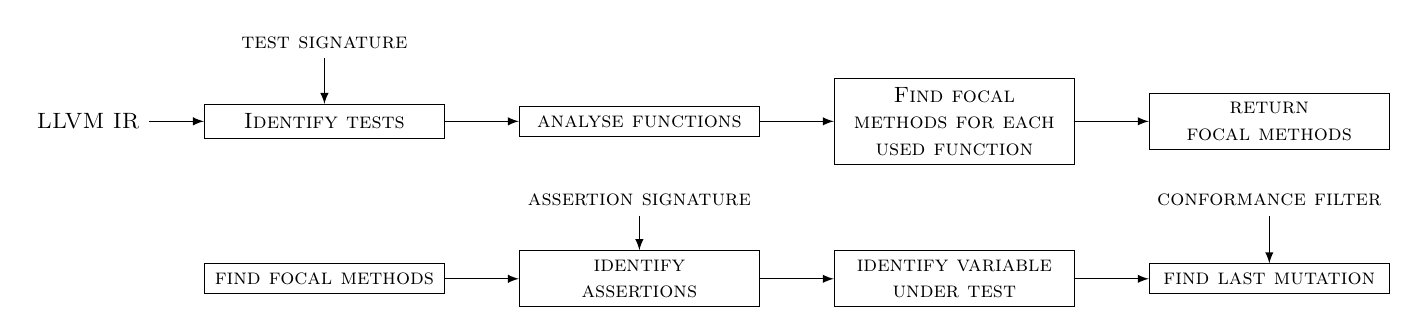
\begin{tikzpicture}[auto, >=latex, node distance = 1.5 cm, font=\footnotesize\scshape]
	\tikzstyle{round} = [draw=black, rectangle, text width=8em, align=center]
	\tikzstyle{invis} = [draw=none]
	
	\node[round] 			at (0, 0) 		(q0) 	{Identify tests};
	\node[round] 			at (4, 0) 		(q1) 	{analyse functions};
	\node[round]			at (8, 0)		(q2)	{Find focal\\methods for each used function};
	\node[round]			at (12, 0)		(q8)	{return\\focal methods};
	\node[invis]			at (-3, 0)		(q3)	{LLVM IR};
	\node[invis]			at (0, 1)		(q4)	{test signature};
	\node[round]			at (0, -2)		(q5)	{find focal methods};
	\node[round]			at (4, -2)		(q6)	{identify\\assertions};
	\node[round]			at (8, -2)		(q9)	{identify variable under test};
	\node[round]			at (12, -2)		(q7)	{find last mutation};
	\node[invis]			at (4, -1)		(q10)	{assertion signature};
	\node[invis]			at (12, -1)		(q11)	{conformance filter};
	
	\path[->]
	(q3)	edge					node		{}	(q0)
	(q4)	edge					node		{}	(q0)
	(q0)	edge					node		{} 	(q1)
	(q1)	edge 					node 		{} 	(q2)
	(q5)	edge					node		{} 	(q6)
	(q6)	edge 					node 		{} 	(q9)
	(q9)	edge					node		{}	(q7)
	(q2)	edge					node		{}	(q8)
	(q10)	edge					node		{}	(q6)
	(q11)	edge					node		{}	(q7);
	\end{tikzpicture}
	\caption{Schematical representation of the approach.}
	\label{approach}
\end{figure*}

With the test methods distinguished from all other methods, we must now analyse those test methods. For each method we will extract all relevant statements, in particular including all invocations and all instructions related to memory modification. For each of the used methods, we will differentiate between assertions and source methods. To do this in a correct way, we will require a secondary input from the user, being the naming convention for assertions, which will also be implied by the testing framework used. We can now analyse the source functions found within the test code, followed by the source functions found within the previous source functions.

To limit the execution time of the analysis, a tertiary depth parameter will be requested from the user, implying the maximal depth for the function evaluation. A depth of 1 would imply that we will only consider the called function body itself as potential for mutations, any subsequently invoked functions will be disregarded. In case a depth of 2 would be given, the body of all methods used within tests, as well as the body of all subsequent methods will be considered and so on. This allows for private methods to still be considered a focal method, even though they might be indirectly invoked via a public function.

Example 1 represents a very simple environment where there is a profile class with corresponding methods, and a single test verifying the \textit{setFirstName} method. For the test to work, an instance of the \textit{Profile} class is needed, as is instantiated on line 16 in the test body. This line is then mutated on line 17 to be retrieved again on line 18. The resulting value will then be compared on line 19. 

Our approach will start by distinguishing the test method defined on line 15 from the other methods (note that there is no notion of classes within LLVM IR, this means that class methods are indistinguishable from other methods). Within this test method's body it will evaluate the invoked methods on line 16, 17 and 18. It will not consider the assertion function on line 19, as it is able to distinguish assertions from other methods.

\subsection{Retrieving the Focal Methods}
In our approach we will distinguish the focal method of a test, by firstly disambiguating between mutators and inspectors, starting from the assertions found within the body of the test function. For each of the variables used within the assertion, the test body will be traced, up until a mutation is found.

The analysis of focal methods will be done by simply tracking the variable under test throughout the invoked methods. During this process, any modification of the memory of the tracked variable will be considered a mutation, and will allow us to mark the top function as a mutator. This means that we are capable of detecting private methods being the actual mutators, even though they are called via a public function. To perform this analysis, we will need an extension, allowing us to disambiguate between public and private functions. We would then simply need to verify whether or not a called function is actually private. In case a called function is private, we will verify whether or not it mutated the variable, in case it is public, it will not be considered, as public functions should have their own test cases. As we are currently unable to detect the difference, all functions are considered as if they are private functions.

For our analysis to work with libraries for which the source code is not given, we will define a third class of invocations, which will be \textit{uncertain}. Method invocations labelled uncertain indicate that the definition of the method is not known due to absence of the actual implementation. Our approach will resolve this by marking the top function as being a potential focal method, but not the only focal method. We would still continue our trace, looking for the first actual mutation that is found, after which both the uncertain method and the last mutator will be returned as being the focal methods of the test.

Finally, an optional focal method conformance filter can be used, which would be a filter to which focal methods must not conform. This is introduced as the language independence has significant effects on the evaluation of focal methods. Without a means for filtering, functions defined within language specific libraries would be considered as being potential focal methods, which greatly reduces the effectiveness of the tool. For example, considering a C++ project, simple assignments of string would be replaced by an assignment function defined within the standard C++ library. This function will never be the intended function under test, but considering a case where strings are compared in an assertion, the last function that will be used to assign said string to a variable will be this string assignment function defined within the std namespace. To prevent this function from being marked as the focal method, analysis of C++ code would benefit greatly from having the std namespace filtered from the set of focal methods. In our analysis, we would then still consider standard library functions as functions leading to a mutation, but not as the top function being the mutator itself.

The application of the filter will also allow us to differentiate between source code and library code and thus detect mutations at the appropriate level. For example, given a function in which a string is assigned, we would not be able to detect this mutation, unless our depth is one level higher, as the mutation would only happen within the body of the string assignment function itself. With the knowledge that this assignment function is not part of the source code, we can allow our approach to evaluate the body of this function, and thus returning the upper function as being a mutator, as this upper function would be within the limits of our max depth.

When going back to the environment represented within Example 1, we can see that we have one assertion, being the invocation on line 19 within the \textit{testSetFirstName} method. This method has two vari-

\begin{sexylisting}{examplary test environment\label{lst:example1}}
class Profile
  firstName
  lastName
	
  method setFirstName(profile, name)
    store name in profile.firstName
  endmethod
	
  method getFirstName(profile)
    var = load firstName from profile
    return var
  endmethod
endclass
	
method testSetFirstName()
  p = Profile()
  p.setFirstName("Ani")
  name = p.getFirstName()
  assertEq(name, "Ani")
endmethod
\end{sexylisting}

\noindent
ables being used, being the constant "Ani", which will not lead to any mutations at all and the name variable. Tracing this name variable upwards, will lead us to the \textit{getFirstName} method, but analysis of the resulting code, will not show any statements that modify memory and it will therefore be flagged as being an inspector. We will also detect that the profile variable was used, which will become our new tracked variable. This very same variable will be used on line 17, and analysis of this function body will show a mutation, being the store on line 6. This means that this function will in fact be flagged as being a mutator, which will end the evaluation for function \textit{testSetFirstName} with the resulting focal method being \textit{setFirstName}.

\section{Case study}
In this section, we will give an example case in which the tool was applied as well as the results obtained from it. Considering the obtained results, we will give an overview in what way these results satisfy our original goal for this research.

\subsection{Stride}
To evaluate the tool, it was applied on a forked and extended version of the original Stride project (version 1.18.06\footnote{\url{https://github.com/broeckho/stride}}), which is a project written in C++. This extended version \footnote{\url{https://github.com/larsvanroy/stride}} includes several additional classes, along with corresponding tests. The tool was applied to the entirety of the test suite, and the used LLVM IR contained compiled versions of all used libraries by the project. This resulted in an LLVM file of which statistics are listed within Table 1. The LLVM IR was generated using the Clang compiler\footnote{\url{https://clang.llvm.org/}}(version 10.0.0).

\begin{center}
	\begin{tabular}{ |p{4.5cm}|p{2.5cm}|  }
		\hline
		lines of code & 3,776,986\\
		\hline
		number of functions   & 54,811\\
		\hline
		number of test functions &   222\\
		\hline
	\end{tabular}
	\captionof{table}{Statistics for the generated LLVM IR code.}
\end{center}

This project was chosen because it is written in a layered manner, where only the most outer layer is accessible. The classes located on the most outer layer will be responsible for all classes directly below them, the classes below the outer classes will be responsible for the classes below those and so on. This structure is interesting, as it implies that test cases testing lower layers must traverse several other classes before arriving at the actual mutation which we want to test, making it an ideal candidate for our approach, as the method under test of those tests will be a private function.

Note that considering the size of the project, the test size may seem very limited, however, many of the functionalities part of the project are not testable on their own, due to the design choices made, and are tested in a more grouped way. 

Furthermore, only the tests regarding the population and generation of data sets were considered for this analysis. The other tests, being utility tests and tests verifying the input and output of data, were tests in which the objects were mutated using public functions. These tests were less interesting for our approach as it has already been proven that the approach is capable of detecting the mutations in such instances. Furthermore, a part of the utility tests were tests in which the method under test was in fact an inspector method, which our approach will never be able to correctly identify. We also disregarded scenario tests, as our approach is specifically intended to identify the method under test in unit tests, as scenario tests often test a list of methods, rather than one single method. The 61 remaining tests are tests in which the method under test is indeed a private function in a lower layer. This selection allows us to more precisely determine the percentage of focal methods we can correctly identify in case a private method is the method under test. If we would not make this selection, the majority of the tests would be tests where the focal method is public, as can be seen in Table 2.

\begin{center}
	\begin{tabular}{ |p{5.5cm}|p{0.5cm}|  }
		\hline
		utility tests & 77\\
		\hline
		input/output tests & 59\\
		\hline
		population and generation tests & 61\\
		\hline
		scenario tests & 25 \\
		\hline
	\end{tabular}
	\captionof{table}{Number of tests of each type within Stride.}
\end{center}

\subsection{Research questions}
A few questions need to be answered to quantify the usefulness of the approach for the given test case. Below is an overview of the questions we attempted to answer using the results of our simulation, alongside an explanation of why this question needs to be asked, and how we intend to find a solution.\\
\\
\noindent
\textbf{Question 1:} \textit{To what extent can we correctly identify the focal methods?}\\
\textbf{Motivation.} Given that the main goal of the tool is to correctly identify the focal methods for a given project, we want to know the percentage of cases in which it is capable of doing so. \\
\textbf{Approach.} We consider the precision and recall of several simulations using different parameters. The precision will be used to determine the percentage of selected focal methods that are actual focal methods. The recall will be used to determine how many of the focal methods we actually find. To allow proper comparisons between approaches, the harmonic mean from both the precision and recall will be considered, computed using the formula below.

\[h-mean = \frac{2 \times precision \times recall}{precision + recall}\]

\noindent
\textbf{Question 2:} \textit{In what way is the depth parameter related to the gain of the tool?}\\
\textbf{Motivation.} The depth parameter is intended to increase the precision of the result, but might also have a negative effect on the recall. It will furthermore have a direct effect on the evaluation time of the analysis. It is important to evaluate the negative effects on the resulting recall to estimate the effect of undefined functions. The execution time is also relevant, as a percentage wise increase in evaluation time will be significant in larger projects.\\
\textbf{Approach.} To test this we will consider the accuracy, recall and evaluation time for all depth values ranging from 0 to 6. By considering the differences between these different simulations we can get an idea of the effect of the depth parameter and from those we can then derive the actual gain of increasing/decreasing the depth. \\
\\
\noindent
\textbf{Question 3:} \textit{In what way can we mitigate the result of language independence?}\\
\textbf{Motivation.} Due to the analysis being language independent, we might incorrectly identify functions as being focal methods. The effect is important to consider to allow for proper comparison with other tools. \\
\textbf{Approach.} To evaluate this, we will consider two different simulation runs, one without a filter and one with a filter, filtering out all functions part of the std namespace. Comparison of the obtained harmonic mean between the two simulations will give us an indication of the gain from removing language specific functionalities from the potential focal methods. The filter that we will use will specifically filter the functions that are part of the standard library of C++ is given below.

\[\text{\small @\_ZNKSt.*?}\mid \text{\small @\_ZNSt.*?}\mid \text{\small @\_ZN9\_\_gnu\_cxx17.*?}\]

\subsection{Results}
Table 3 visualises the results obtained from the simulation. For each of the considered depths it gives the precision, recall, mean and time it took to run the simulation. For each depth we ran two different simulations, one without a filter and one with a filter, filtering out just the methods part of the C++ standard library. Note that we only gave simulations up to depth 6, as 5 was the maximal depth to which the considered tests reached. This was verified by running up to depth 10 where we would have an increase in simulation time, but the precision, recall and mean would not change.

\begin{table*}[t]
	\centering
	\begin{tabular}{ |c|c|c|c|c|c|c|c|  }
		\hline
		\multirow{2}{*}{filter applied} & \multirow{2}{*}{parameter} & \multicolumn{6}{|c|}{depth} \\
		\cline{3-8}
		& & 1 & 2 & 3 & 4 & 5 & 6\\
		\hline
		\multirow{4}{*}{yes} & precision & 0.36 & 0.36 & 0.4. & 0.43 & 0.58 & 0.58\\
		\cline{2-8}
		& recall & 0.39 & 0.39 & 0.52 & 0.52 & 0.77 & 0.77\\
		\cline{2-8}
		& mean & 0.38 & 0.38 & 0.47 & 0.47 & 0.66 & 0.66\\
		\cline{2-8}
		& time & 68.35 s &  70.61 s & 78.43 s  & 79.81 s & 98.19 s & 103.51 s \\
		\hline
		\multirow{4}{*}{no} & precision & 0.0 & 0.28 & 0.46 & 0.46 & 0.55 & 0.55\\
		\cline{2-8}
		& recall & 0.0 & 0.31 & 0.52 & 0.52 & 0.72 & 0.72\\
		\cline{2-8}
		& mean & 0.0 & 0.29 & 0.49 & 0.49 & 0.62 & 0.62\\
		\cline{2-8}
		& time & 71.49 s &  71.08 s & 73.94 s & 79.51 s & 97.78 s & 105.43 s\\
		\hline
	\end{tabular}
	\captionof{table}{Statistics for the generated LLVM IR code for tests related to generation and population.}
\end{table*}

\noindent
\textbf{Question 1:} \textit{To what extent can we correctly identify the focal methods?}\\
Over all 12 simulations, the lowest encountered recall is 0\%, which happens when we do not apply a filter at depth 1, this is a result of our analysis assuming that all code is source code and any code part of the standard library part of C++ is therefore not analysed if it is outside of the max depth. When we do add it to our filter, we can see that the minimal recall is equal to 39\%, which is much higher, as we now know that the standard library functions are not part of the source code. We can therefore analyse these functions without regard to our maximal depth. A recall equal to 39\% is equal to the recall we would obtain without considering any depth, and is therefore the recall that would be obtained if using the approach specific for public methods.

When we increase the depth, our recall goes as high as 77\% which signifies that the approach is capable of correctly determining the focal methods. The reason that this only occurs at such a high depth, is because of the layered structure that is used by this tool. The reason that lower depths give a far lower recall, is because part of the test methods effectively have their focal method, i.e. their mutation, at 5 invocations deep. In case the depth variable is not as high, the actual mutation will never be considered, and the functions will just be marked as being an inspector.

The low precision is due to us incorrectly labelling functions as being a mutator due to the actual mutator not being discoverable. As soon as the actual focal method becomes discoverable, no earlier functions will be considered and this leads to an increase in precision, as can be seen in the table above. In a few cases, an extra mutator was found due to our language independent approach not allowing us to distinguish between expected value and value under test. This means that we often get two focal methods for a single assertion, where most cases will only have one variable that was actually under test. An additional parameter indicating the parameter location within an assertion (e.g. the asserted variable is the second variable in an assertion) might resolve this for projects in which a standard is used for this, but this once again requires developers to uphold a convention, which is one of the things we intended to avoid using this approach. Simple assumptions regarding order of mutations would also be invalid, as it might be that the oracle against which we compare, is an object created via a library function. In this case our filter will not filter it out, and it might be initialised after the actual focal method occurred (just before the oracle evaluation).

The cases in which the focal method was not found at all were cases where a no throw assertion was used or cases where a mutation occurred after our focal method, which was not the method under test. The cases where a later mutation occurred where cases where an iterator of a locally defined type, being \textit{CSV}, was used. In these cases we would iterate over the modified object, and rather than the mutation (which occurred just before the loop), the update of the iterator would be flagged as being the actual mutation. In the cases where a no throw assertion was used, the tool has no capability of detecting what the function under test was, as there is no variable to track through the code. Considering the 61 tests that were evaluated, in 14 of the tests the focal method was incorrectly identified, of which 8 were due to a no throw assertion and 6 due to a mutation occurring after the method under test as can be seen in Table 4.

\begin{center}
	\begin{tabular}{ |p{6.5cm}|p{0.5cm}|  }
		\hline
		number of tests & \hfil61 \\
		\hline
		correct focal method & \hfil47\\
		\hline
		incorrect due to no throw assertion  & \hfil8\\
		\hline
		incorrect due to later mutation & \hfil6\\
		\hline
	\end{tabular}
	\captionof{table}{Overview for the number of correctly identified methods under test.}
\end{center}

\noindent
\textbf{Question 2:} \textit{In what way is the depth parameter related to the gain of the tool?}\\
When comparing the simulation for depth 1 compared to depth 6, we can see a definite increase in the mean parameter. This is expected to happen, as a higher depth means that we can correctly identify focal methods which lie several invocations deep. 

While this increase in mean is exactly what we wanted, we must also consider the increase in simulation time. Up to a depth of 6, the simulation time increased by about 50 \% for both simulation types. This is a clear indication that even though the depth does have an impact on the simulation time, it should not be limited purely due to this, and should be based on the structure of the project.

\noindent
\textbf{Question 3:} \textit{In what way can we mitigate the result of language independence?}\\
When comparing the results from the simulations where the filter was applied, to the results where the filter was not applied, we can definitely see an improvement in both precision and recall. Note that the mean is higher or equal for all simulations of equal depth, in favour of the simulation using a filter. This indicates that the use of a filter definitely has a positive effect on the quality of the results.

\section{Threats to validity}
We note a number of threats to the validity of the found results.

A primary remark should be that we did not consider multiple languages, even though this is a language independent tool. This remark is correct, in the sense that we should have performed analysis on bigger and more diverse projects, although that the analysis is fully language independent. We analysed a semi large LLVM IR file which contained the majority of the possible LLVM IR statements. The approach managed to analyse this correctly, and gave results based upon this. In this approach, no language specific components should have been present, other than the input from the user itself, and this input is possible for any chosen programming language. 

Secondary, we need to consider that we did not write all of these tests and there is a human error present in the sense that we manually determined the correct result of the tool. However, we believe that the we correctly identified the actual goals of the tests, and thereby correctly assumed the intended focal method.

Another threat that needs to be considered, is the fact that we need the entire source of every library used to be able to correctly analyse the code. In most cases, the source code of libraries should be available online, but this is not always guaranteed. For example, cases where the library is considered proprietary, might not make their source code readily available. In these cases, the quality of the result will be reduced, as all functions directly using this library, will be marked as being uncertain, given that the invocation to the library function occurs inside the given max depth. This could lead to a decrease in precision, as all functions accepting the variable under test would be marked as being potential mutators (given that they occur before an actual recognisable mutation).

We must also consider the fact that we are unable to correctly identify the method under test in cases where the method under test is an inspector. Our approach will never identify an inspector as being the method under test, and our approach will therefore fail in these cases. 

Other than the previous remarks, this analysis is not dependent on any conventions to which developers need to adhere nor did we consider the help of any outside tools. We should therefore not undergo any accumulative error from such sources.

\section{Future work}
As we originally aimed to correctly identify private methods being a focal method, there should be an extension to the analysis, which feeds it information regarding which method is private and which method is not. As it currently stands it is perfectly capable of analysing focal methods at a lower depth, but it is unable to determine whether or not this chain consisted out of private methods, or whether or not public methods occurred along the chain. In case one of the subsequent steps contained a public method, this chain is not valid, and should be disregarded as a candidate for focal method, as the public method should be tested separately.

There also needs to be an extension to easily allow users to determine namespaces defined by a library. We do not want library functions to be the function under test, but as a user it is hard to know what namespaces should be excluded, as this requires an in depth analysis of library code. An extension capable of simply analysing the used namespaces, given that the library source is present, would allow users to greatly enhance their analysis.

Cases where the method under test is not a mutator will also be incorrectly classified. This is an issue to which the current approach is not suitable. A different approach for functions in which the function under test is an inspector need to be considered to resolve this.

\section{Conclusion}
In this paper, we presented a new automated method to determine test-to-code traceability links using focal methods. The focal methods allowed us to determine a link from test code to their tested methods.

We were able to show that this approach is indeed capable of detecting focal methods, by applying the approach to Stride. Considering this example, we were able to correctly identify the method under test in 77\% of the cases, with a precision of 58\%. The test cases in which the test method was not detected, where cases where mutations occurred after the method under test, or cases where no throw assertions where used. In these cases, the considered approach was unable to correctly identify the method under test.

While the results of the experiment were promising, there is still need for further improvements. For this paper, we only considered one project, which only covered one language. This being a language independent approach, further evaluation of different languages should be performed, before fully concluding that this approach is capable of analysing all major programming languages in a language independent way.

\printbibliography
\end{multicols}
\end{document}